% Supplementary material (appendix) of the MLSys 2027 submission, compiled on
% its own for the separate appendix upload. Same preamble as main.tex.
\documentclass{article}
\usepackage{microtype}
\usepackage{graphicx}
\usepackage{booktabs}
\usepackage{amsmath,amssymb}
\usepackage{xcolor}
\usepackage{multirow}
\usepackage{array}
\usepackage{hyperref}
\newcommand{\theHalgorithm}{\arabic{algorithm}}
\usepackage{mlsys2025}
\mlsystitlerunning{Supplementary material: When FLOPs Point the Wrong Way}
\newcommand{\aslot}[1]{\textcolor{red}{[A100: #1]}}
\newcommand{\rstar}{r^{*}}
\newcommand{\Efact}{E_{\mathrm{fact}}}
\newcommand{\Edense}{E_{\mathrm{dense}}}
\newcommand{\us}{\,\mu\mathrm{s}}

\begin{document}

\twocolumn[
\mlsystitle{Supplementary Material: When FLOPs Point the Wrong Way: Pre-Registered Energy Crossovers for Low-Rank Inference on GPUs}
\begin{mlsysauthorlist}
\mlsysauthor{Anonymous Authors}{anon}
\end{mlsysauthorlist}
\mlsysaffiliation{anon}{Anonymous Institution, Anonymous City, Anonymous Country}
\mlsyscorrespondingauthor{Anonymous Author}{anon.email@example.com}
\vskip 0.3in
]

\printAffiliationsAndNotice{}

Table and figure numbers below continue the main paper's numbering only within this document; cross-references to the main paper are by section.

% Appendix of the MLSys 2027 submission. Included by main.tex unless \NOAPPENDIX is
% defined, and compiled on its own by supplementary.tex for the separate upload.
\appendix
\section{Instrumentation gate details}
\label{app:gate}

Table~\ref{tab:gate_detail} lists the gate measurements behind Table 1 of the main paper. On the laptop the counter advanced by 26.0 kJ over the 55 s pre-heat idle window against 242 J from the integrated 4.4 W power reading, reported 1.514 J per call against 1.015 J for the capped GEMM blocks (CV 4.2 against 0.32 percent), and 2.89 mJ against 1.107 mJ for the dispatch loop. The window-sufficiency sweep (six lengths from 0.5 to 20 s, five randomized repetitions each) gave a smallest sufficient length of 0.5 s for the capped GEMM on both platforms (a timing measurement at a pinned power) and 20 s for the dispatch loop on the laptop; on the A100 no length met the 2 percent target for the dispatch loop because the sweep ran while the die cooled from the 395 W sequence (a 2.4 percent trend over 100 s), which is why every later window on both platforms is preceded by thermal settling under load.

\begin{table}[h]
\caption{Gate measurements on the two platforms (full runs \texttt{20260915T164645} and \texttt{20260925T064203}).}
\label{tab:gate_detail}
\vskip 0.1in
\centering
\footnotesize
\begin{tabular}{@{}p{3.3cm}p{2.3cm}p{2.3cm}@{}}
\toprule
Quantity & Laptop & A100 \\
\midrule
Power limit (enforced) & 175 W & 400 W \\
Idle power, pre-heat (55 s) & 4.40 W, drift $-0.62$ W/min & 79.1 W, drift $-2.2$ W/min \\
Hot-idle bias after settling & $+0.006$ W & $+0.88$ W \\
Heat load, 60 s & 171.7 W, 74 C max & 379.5 W, 66 C max \\
Thermal settle after heat load & 16 s & 14 s \\
Power reading update period & 500 ms & 103 ms (20 ms native) \\
Counter update period & 100 ms & 101 ms \\
Capped GEMM, 10 blocks & 1.015 J/call, CV 0.32\% & 2.853 J/call, CV 0.80\% \\
Dispatch loop, 10 blocks & 1.107 mJ/call, CV 1.99\% & 1.159 mJ/call, CV 1.10\% \\
Dispatch loop, time and power per call & 14 to 19$\us$, 60 W & 9.9$\us$, 116 W \\
SM clock under the loop & 2325 MHz & 1410 MHz \\
Windows, samples & 83, 14877 & 83, 15436 \\
\bottomrule
\end{tabular}
\end{table}

\section{Held-out crossover cells and model parameters}
\label{app:tables}

Table~\ref{tab:cells} lists the 14 held-out $(d, B)$ cells per platform with the measured crossover, the M1 prediction, and whether the point rule (same verdict kind and $\rstar$ within a factor of 1.5) is met. The M3 parameter vectors are, for the laptop: $t_{\mathrm{launch}} = 16.6\us$, BW $= 443$ GB/s, $R = 8.70$ TMAC/s, $p_{\mathrm{floor}} = 46.4$ W, $p_{\mathrm{memory}} = 174.6$ W, $p_{\mathrm{compute}} = 183.7$ W; for the A100: $t_{\mathrm{launch}} = 13.2\us$, BW $= 1071$ GB/s, $R = 7.37$ TMAC/s, $p_{\mathrm{floor}} = 100.8$ W, $p_{\mathrm{memory}} = 362.4$ W, $p_{\mathrm{compute}} = 364.5$ W. Both fits are joint on energy and per-call time with the powers ordered within the cap, from 54 starting points, selected by the lowest cost.

\begin{table}[h]
\caption{Held-out cells: measured $\rstar$, M1 prediction, point-rule outcome. "dense" means dense wins at every tested rank.}
\label{tab:cells}
\vskip 0.1in
\centering
\footnotesize
\setlength{\tabcolsep}{4pt}
\begin{tabular}{@{}lrrrcrrc@{}}
\toprule
 & \multicolumn{3}{c}{Laptop} & & \multicolumn{3}{c}{A100} \\
\cmidrule{2-4} \cmidrule{6-8}
$(d, B)$ & meas. & M1 & hit & & meas. & M1 & hit \\
\midrule
(1024, 1) & 202 & 206 & yes & & 293 & dense & no \\
(1024, 4) & 374 & 220 & no & & dense & 54 & no \\
(1024, 16) & 268 & 263 & yes & & dense & 92 & no \\
(1024, 64) & 335 & 343 & yes & & 208 & 212 & yes \\
(1024, 256) & 344 & 426 & yes & & 492 & 400 & yes \\
(1024, 1024) & 454 & 464 & yes & & 449 & 492 & yes \\
(1024, 4096) & 484 & 476 & yes & & 455 & 499 & yes \\
(4096, 1) & 2034 & 1972 & yes & & 2032 & 2048 & yes \\
(4096, 4) & 1723 & 1975 & yes & & 1868 & 1725 & yes \\
(4096, 16) & 1908 & 1978 & yes & & 1875 & 1834 & yes \\
(4096, 64) & 2203 & 1995 & yes & & 1947 & 1954 & yes \\
(4096, 256) & 1698 & 2007 & yes & & 2061 & 2013 & yes \\
(4096, 1024) & 1912 & 2011 & yes & & 1818 & 2032 & yes \\
(4096, 4096) & 2012 & 2015 & yes & & 2133 & 2038 & yes \\
\bottomrule
\end{tabular}
\end{table}

\section{Additional figures}
\label{app:figures}

\begin{figure}[h]
\centering
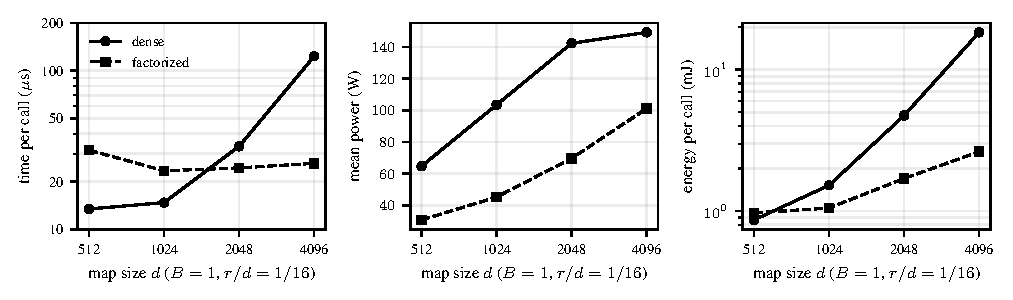
\includegraphics[width=\columnwidth]{figures/regimes_laptop.pdf}
\caption{Per-call time, mean power, and energy at $B = 1$ and $r/d = 1/16$ on the laptop GPU. The dense matrix-vector product sits on a 14$\us$ launch floor at reduced power up to $d \approx 1024$ and becomes memory bound above it; the factorized form pays two launches and saves energy only once the dense form is streaming weights.}
\label{fig:regimes}
\end{figure}

\begin{figure}[h]
\centering
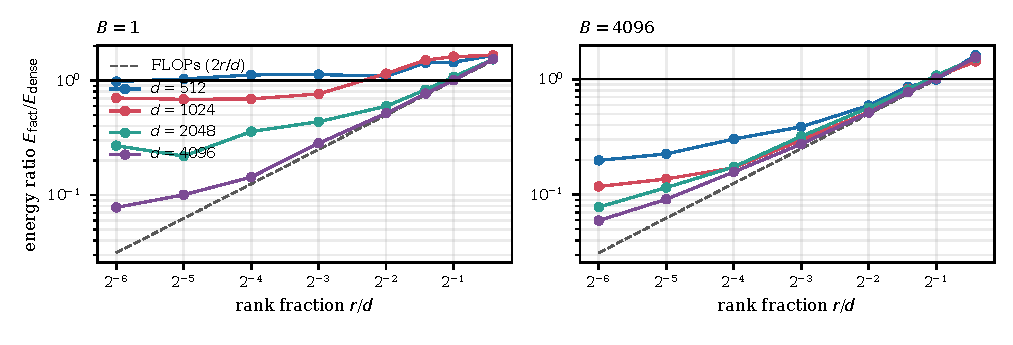
\includegraphics[width=\columnwidth]{figures/ratio_vs_rank_laptop.pdf}
\caption{Laptop GPU: energy ratio against rank fraction at $B = 1$ (left) and $B = 4096$ (right).}
\label{fig:ratio_laptop_full}
\end{figure}

\begin{figure}[h]
\centering
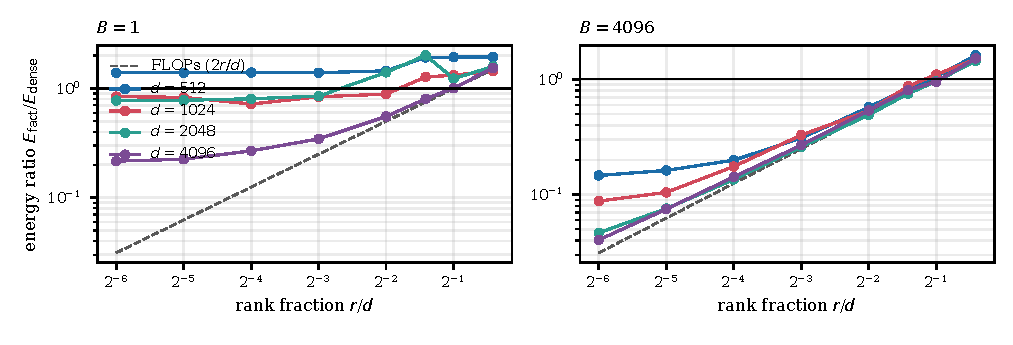
\includegraphics[width=\columnwidth]{figures/ratio_vs_rank_a100.pdf}
\caption{A100: energy ratio against rank fraction at $B = 1$ (left) and $B = 4096$ (right).}
\label{fig:ratio_a100_full}
\end{figure}

\begin{figure}[h]
\centering
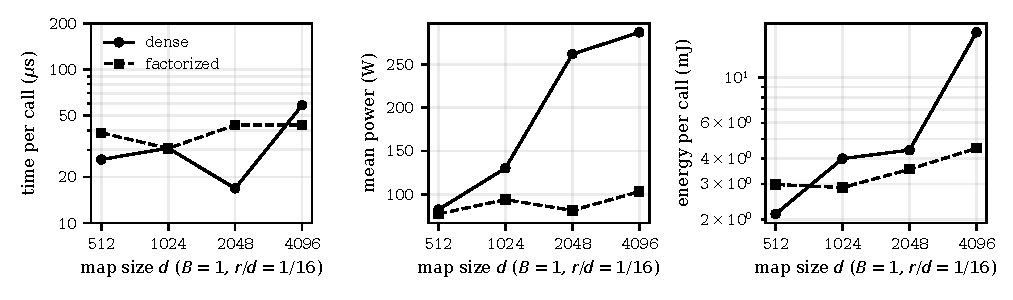
\includegraphics[width=\columnwidth]{figures/regimes_a100.pdf}
\caption{A100: per-call time, mean power, and energy at $B = 1$ and $r/d = 1/16$. Unlike the laptop (Figure~\ref{fig:regimes}), the dense call at $d = 2048$ is faster than at $d = 1024$ because cuBLAS switches from a split-K kernel plus a reduction to a single memory-bound kernel.}
\label{fig:regimes_a100}
\end{figure}


\end{document}
